\section{Exploring the Data}
\label{sec:Exploring the Data}

\subsection{Relationships Dataset}

%\subsection{Terror Attacks Dataset}
%\begin{figure}[H]
%\begin{center}
%\includegraphics[width=\textwidth]{../subGraph.png}
%\caption{}
%\label{fig:}
%\end{center}
%\end{figure}

\begin{figure}[H]
\begin{center}
    \begin{subfigure}[b]{0.45\textwidth}
        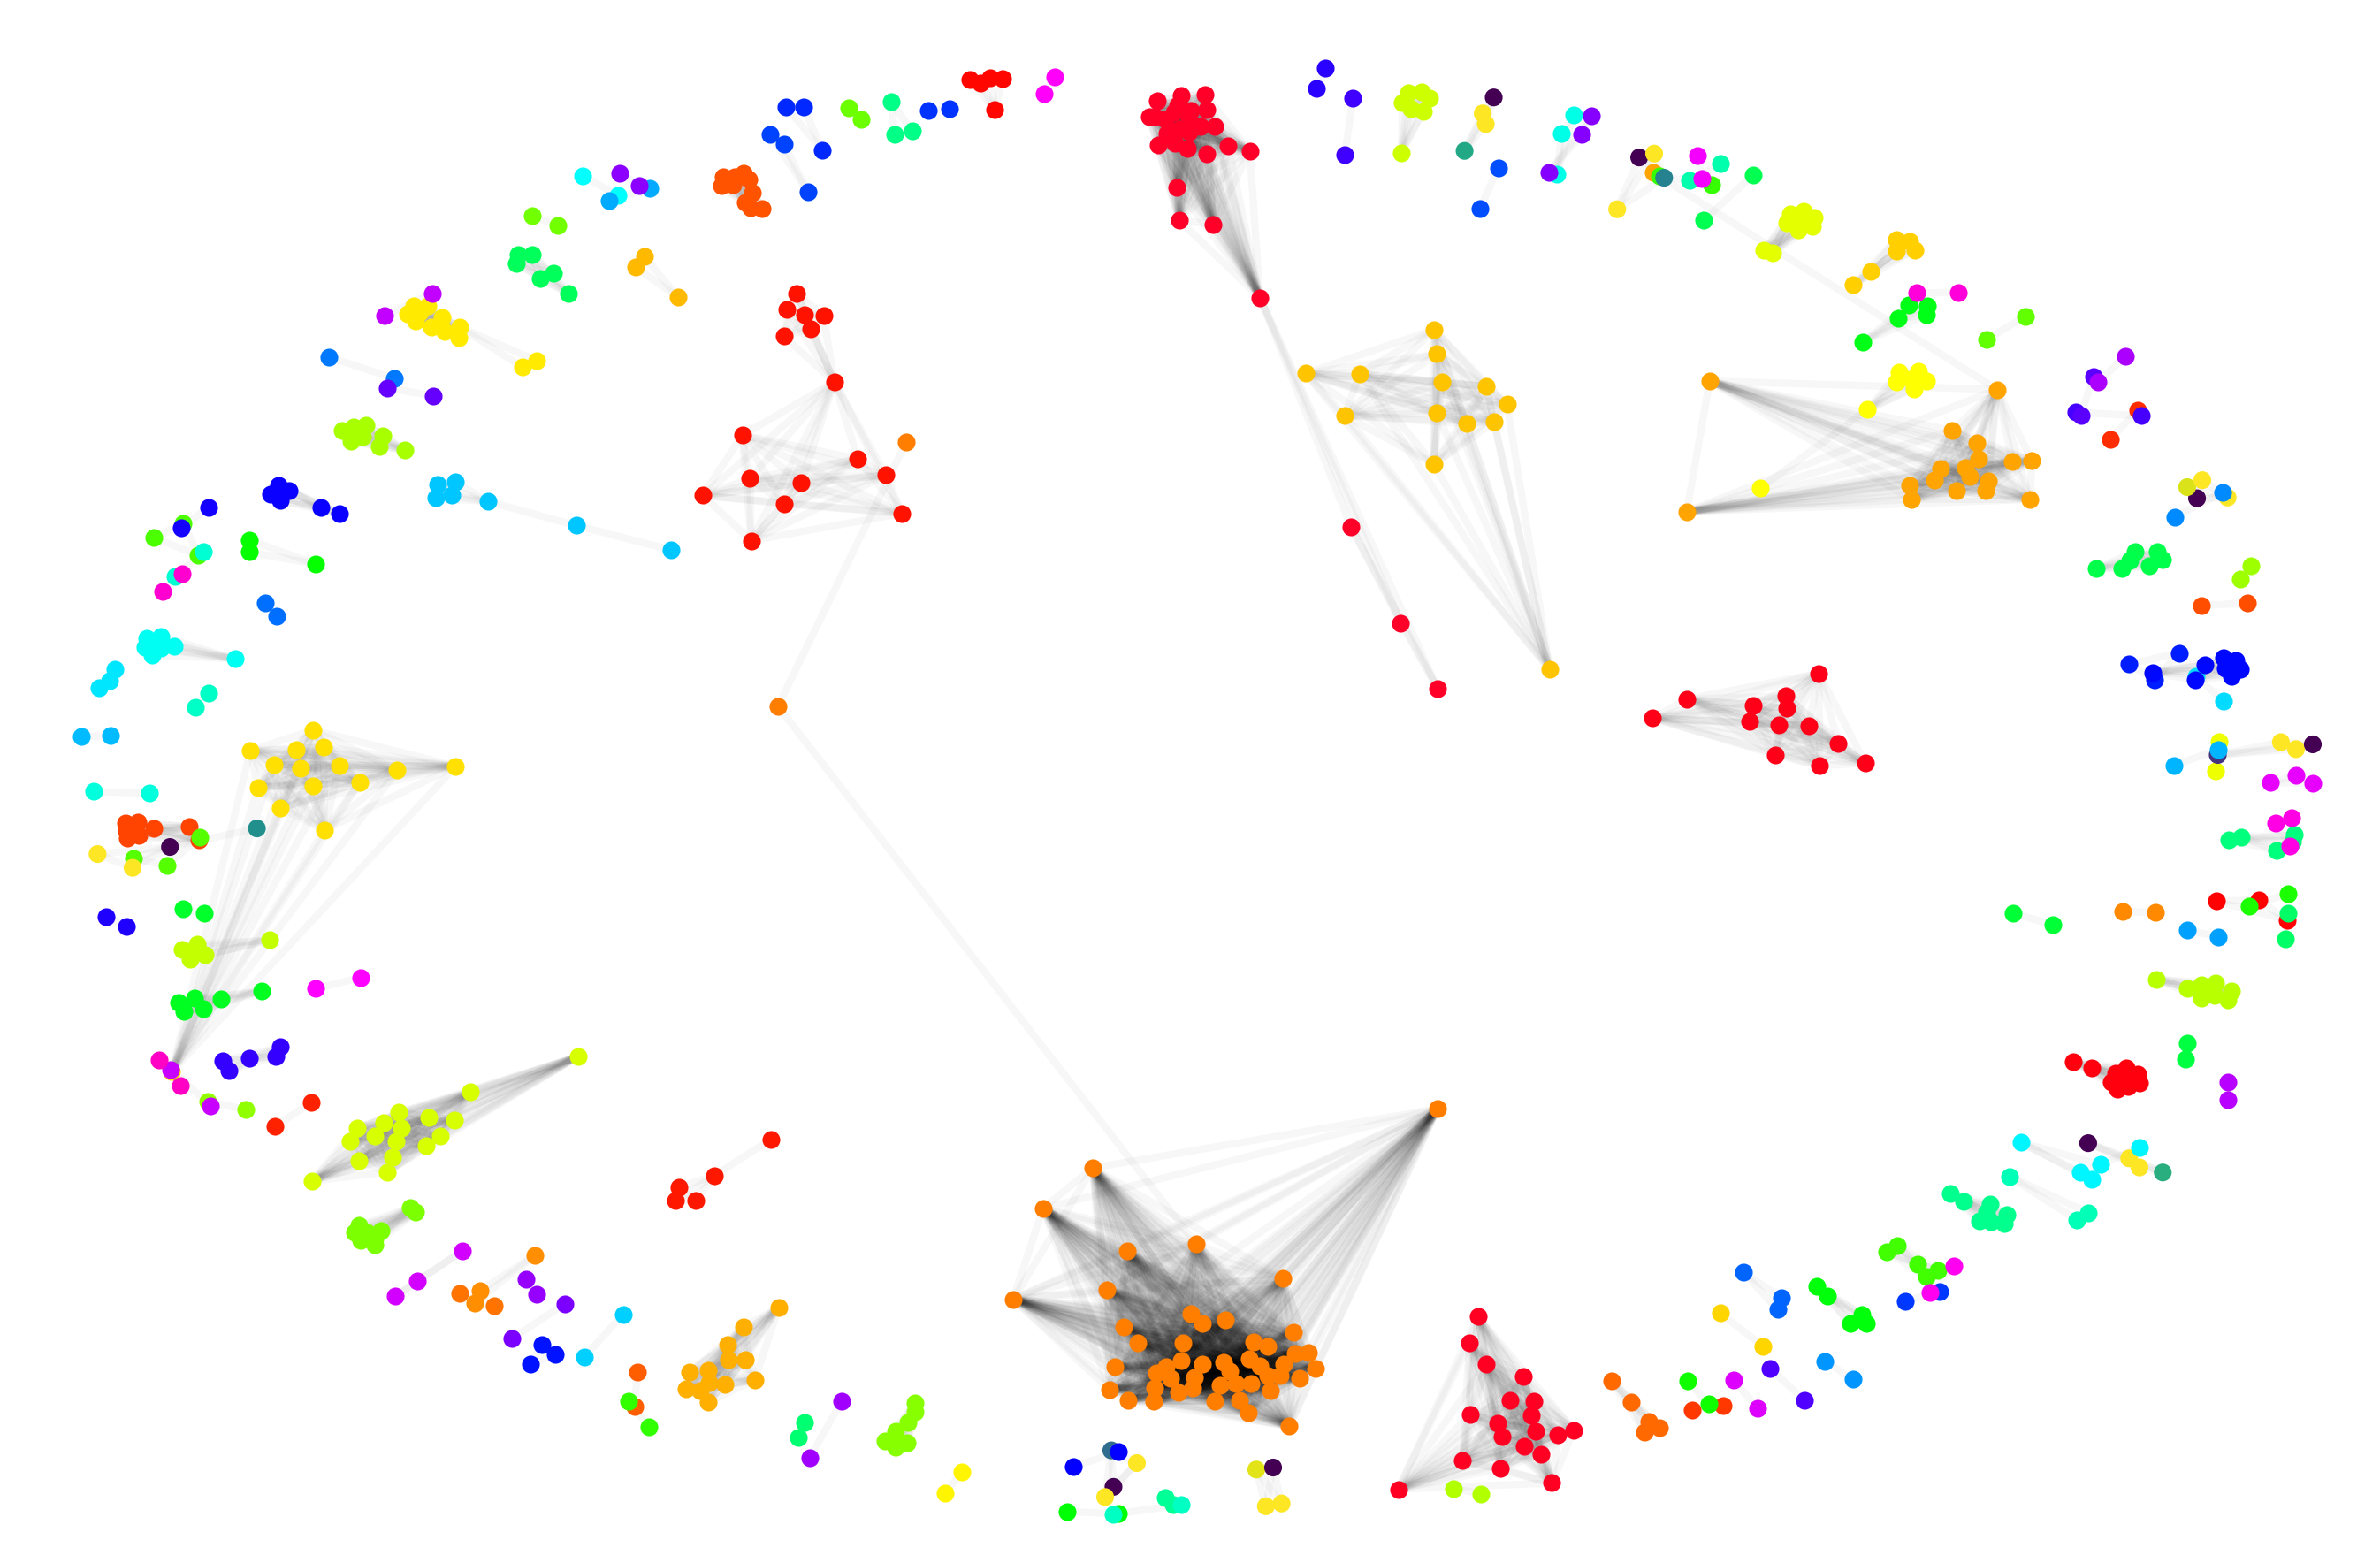
\includegraphics[width=\textwidth]{graphLoc.png}
        \caption{Terror attacks location graph, colouring by component ID}
        \label{fig:graphLoc}
    \end{subfigure}
    ~
    \begin{subfigure}[b]{0.45\textwidth}
        \includegraphics[width=\textwidth]{subGraph.png}
        \caption{Ten biggest components from the terror attacks location graph}
        \label{fig:subGraph}
    \end{subfigure}
\caption{Graphs analysed in the project}
\label{fig:graphPlots}
\end{center}
\end{figure}

%\begin{align}
%w:~		\mathcal{N}^2 &\to \mathcal{R} \\
%(n_1,n_2)				&\mapsto \alpha_1 l_{n_1,n_2}+\alpha_2 \left(\exp\left(-\frac{\| n_1-n_2\|}{\max_{n_i,n_j\in\mathcal{N},i\neq j}\| n_i-n_j\|}\right)-\exp(-1)\right)
%\end{align}
